\section{Fase 4: Análisis Exploratorio de datos oncológicos}

En esta fase, el científico de datos obtiene el conjunto de datos o imágenes que fueron organizados previamente por el ingeniero de datos y realiza un \textit{Análisis exploratorio de datos} para descubrir patrones generales en la información generada. Cabe resaltar, que en esta fase el acompañamiento del medico experto en oncología es de vital importancia, ya que los datos o imágenes que van ser explorados por el científico pueden contener variables que pueden tener o no un valor significativo para el experto, ayudando así a determinar si el análisis planteado para responder la pregunta va o no por un buen camino, de modo que es posible que se agreguen o eliminen diversas variables para lograr el resultado esperado. Adicionalmente, es necesario que los diversos análisis generados estén apoyados con gráficas que sean entendibles por todo el \textit{Data Analysis Team}, esto con el proposito de aportar ideas, y desde esta fase ir encontrando posibles correlaciones entre las variables oncológicas.

Se debe agregar, que en esta fase se abarcan todas las actividades para construir el conjunto de datos o imágenes que se utilizará en la siguiente etapa de modelado y ejecución. Entre las actividades se encuentran el procesamiento y transformación de datos oncológicos, en donde es necesario realizar la limpieza de datos, combinar datos de múltiples fuentes y transformar los datos en variables de valor. En esta fase, es importante el trabajo en equipo y la comunicación continua entre el ingeniero y el científico de datos para tratar los valores no válidos o faltantes, eliminar duplicados, dar un formato adecuado y combinar archivos, tablas y plataformas. Adicionalmente, el medico experto en oncología deberá proporcionar un visto bueno para proceder con la siguiente fase. Esto dado que al ser experto en el tema de dominio tiene un conocimiento mas profundo de las variables o imágenes que esta observando, y si existiese información innecesaria para el diagnostico del cáncer de mama es posible depurar dicha información para que no afecte el entrenamiento y posterior ejecución del modelo de ML y DL.

\subsection{Análisis Parcial de datos crudos}
En primer lugar, se realizó un análisis parcial del conjunto de datos \textit{“Breast Invasive Carcinoma (TCGA, Cell 2015)”} para conocer su composición inicial(cruda) y así poder identificar los registros que deben ser eliminados, transformados ó imputados. Cabe resaltar, que esta etapa es propuesta como parte de esta investigación para los datos de tipo genómico relacionados cáncer de mama. Lo anterior, debido a que el \textit{EDA\footnote{Exploratory Data Analysis}} tradicional parte del análisis descriptivo, y en este caso los tipos de datos son obtenidos de diferentes fuentes medicas las cuales no presentan una estructura fija ni estandar  en la informacion recopilada de los pacientes que padecen esta enfermedad, por lo que seria incorrecto realizar un análisis sobre datos que dada su estructura y forma generan informacion errónea. En la figura \ref{EDA} se puede observar las composición estadística unidimensional de la 110 variables, las cuales permitieron identificar el comportamiento inicial de los datos. Con base a las gráficas obtenidas, se genero el siguiente análisis: 

\begin{itemize}[label=\HandPencilLeft]
	\item El conjunto de datos esta conformado por 95 variables \textit{Categóricas} y 15 variables \textit{Numéricas}.
	
	\item Dada la naturaleza de las preguntas planteadas en el BCQM en donde se busca la identificación de características genéticas, las variables \textit{Study ID, Patient ID, Sample ID, Other Patient ID, Other Sample ID, Form completion date y Pathologyc Report File Name} no generan un aporte significativo para encontrar una respuesta de valor, dado lo anterior fueron eliminadas del conjunto de datos con el cual se entrenaron a los modelos de ML.
\end{itemize}

\newpage
\begin{figure}
	\centering
	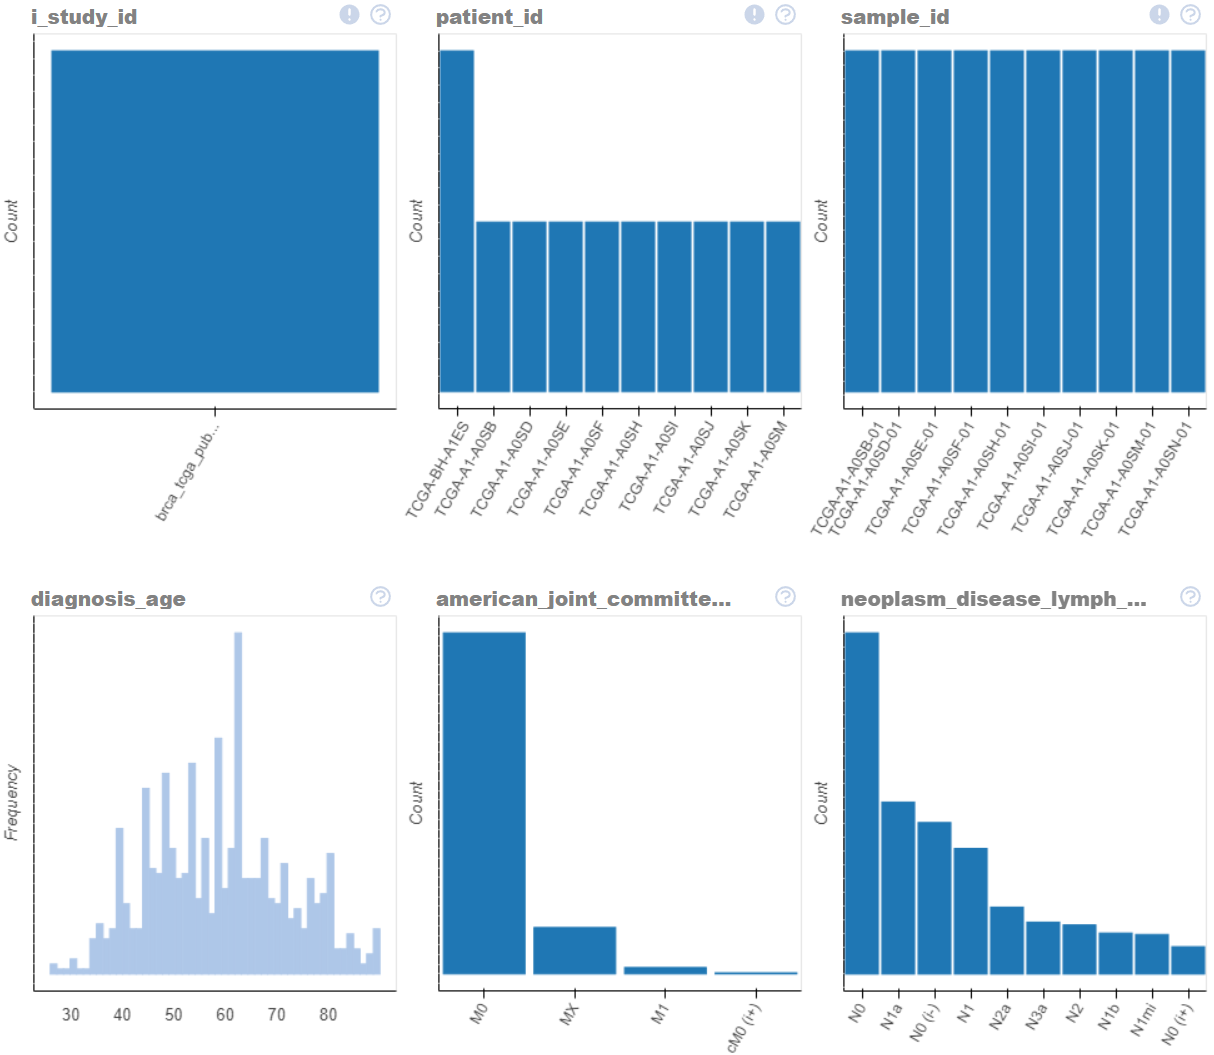
\includegraphics[width=1
	\linewidth]{NOTEBOOK/IMAGES_EDA/1}
\end{figure}

\begin{figure}
	\centering
	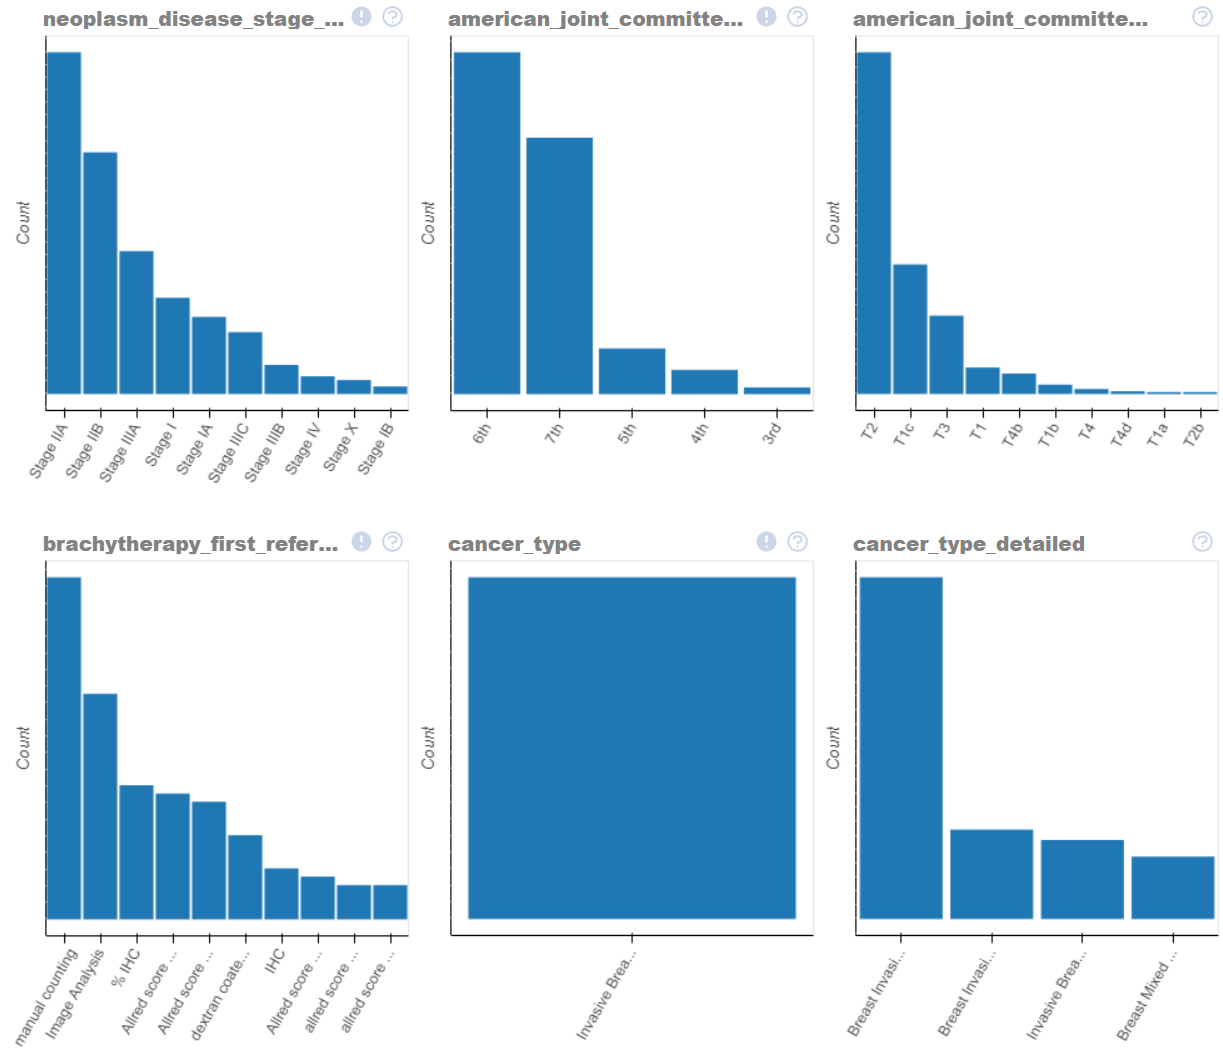
\includegraphics[width=1
	\linewidth]{NOTEBOOK/IMAGES_EDA/2}
\end{figure}

\begin{figure}
	\centering
	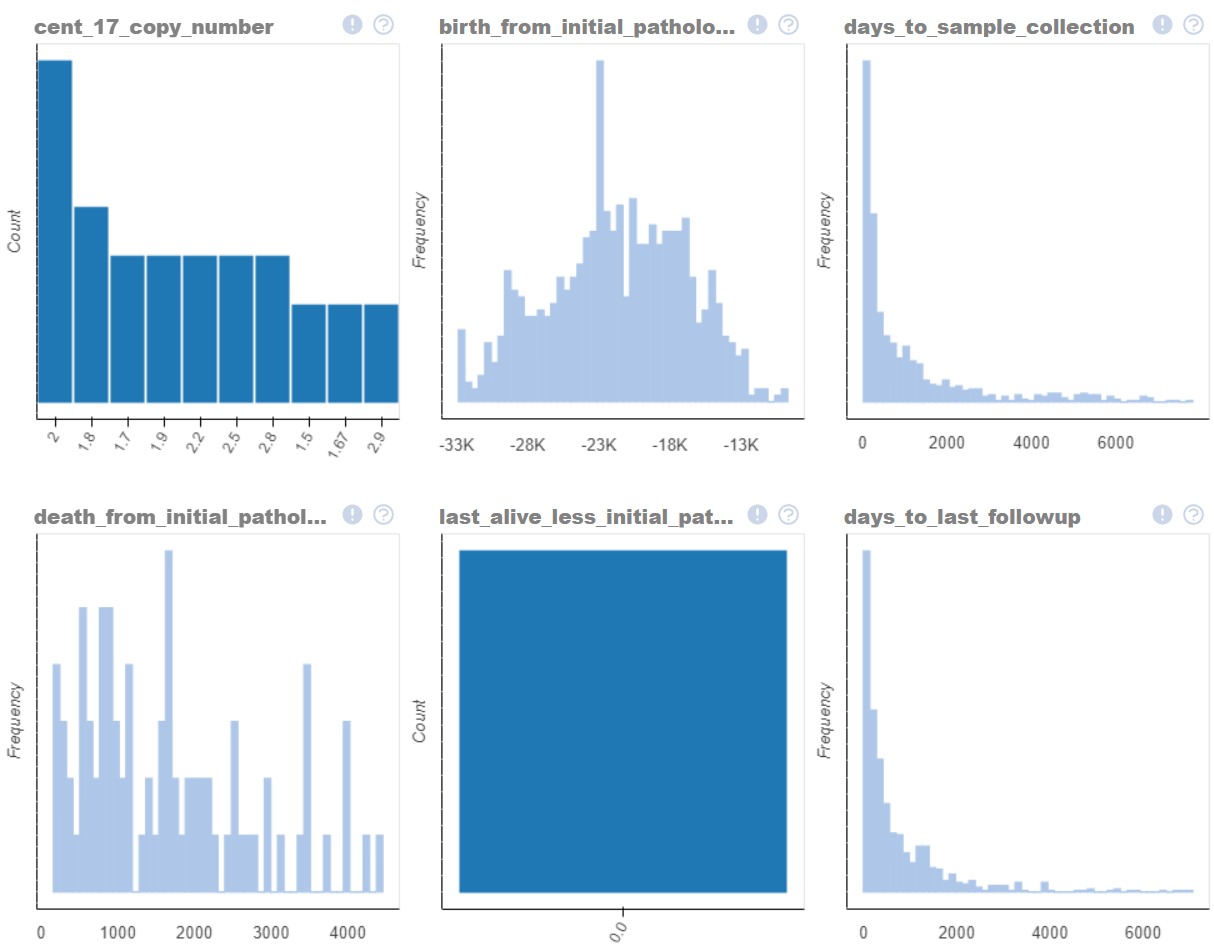
\includegraphics[width=1
	\linewidth]{NOTEBOOK/IMAGES_EDA/3}
\end{figure}

\begin{figure}
	\centering
	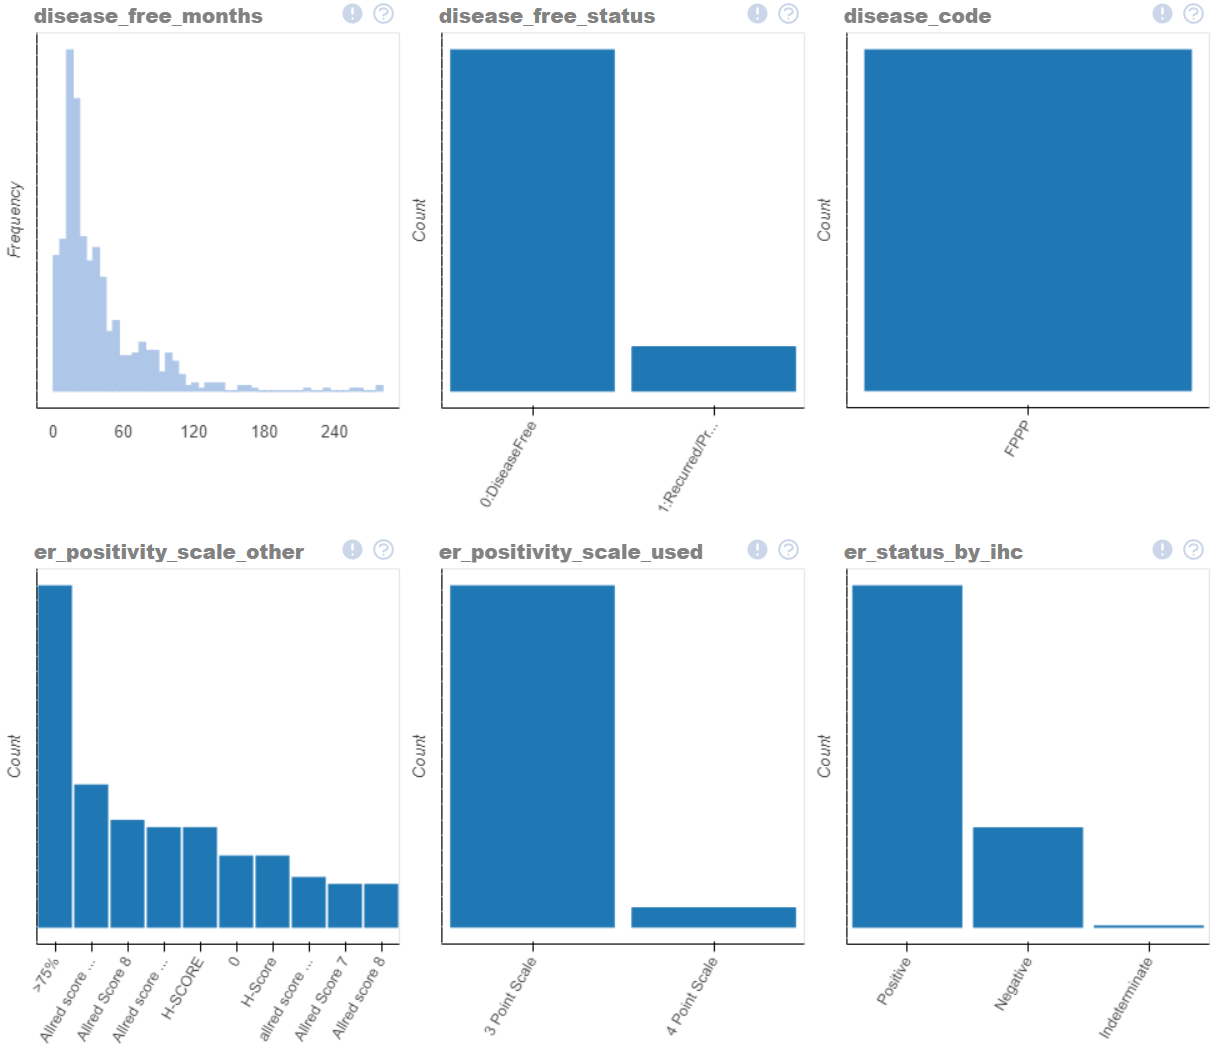
\includegraphics[width=1
	\linewidth]{NOTEBOOK/IMAGES_EDA/4}
\end{figure}

\begin{figure}
	\centering
	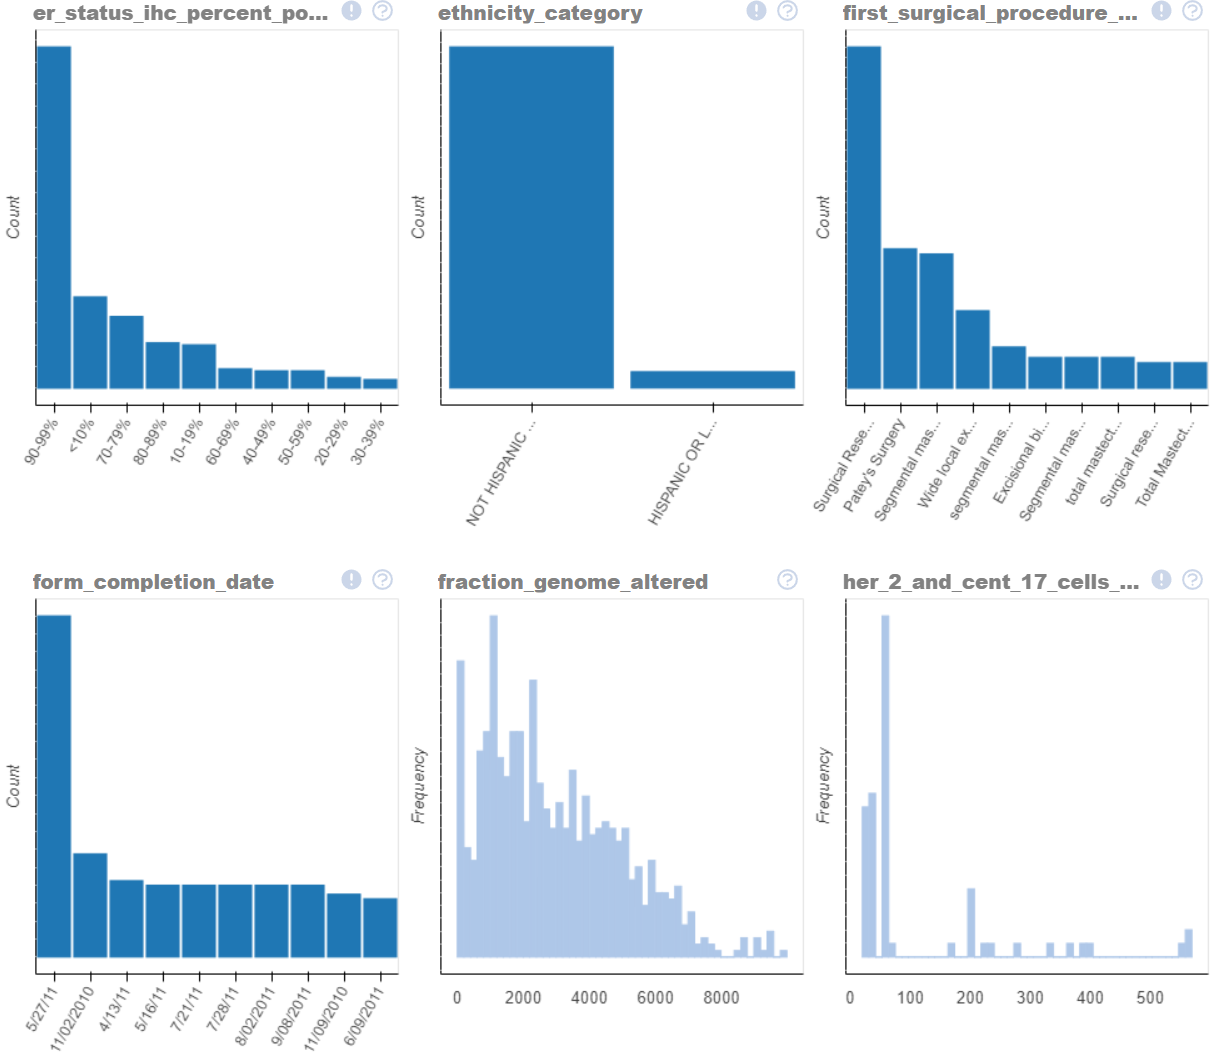
\includegraphics[width=1
	\linewidth]{NOTEBOOK/IMAGES_EDA/5}
	\label{EDA}
	\caption{Distribución del conjunto de datos del Carcinoma invasivo de mama.}\label{fig:foobar}
\end{figure}


\subsection{Detección de datos Ausentes}
En segundo lugar, basados en la obtención de los atributos del conjunto de datos \textit{“Breast Invasive Carcinoma (TCGA, Cell 2015)”}, se realizo un análisis de la cantidad de datos perdidos para identificar las variables y en la etapa posterior realizar la limpieza y el pre-procesamiento de los datos de destino hacerlos consistentes y sin ningún tipo de ruido. Los resultados obtenidos se pueden observar en la figura \ref{Missing_Bar_Chart}:


\begin{figure}[!htb]
	\centering
	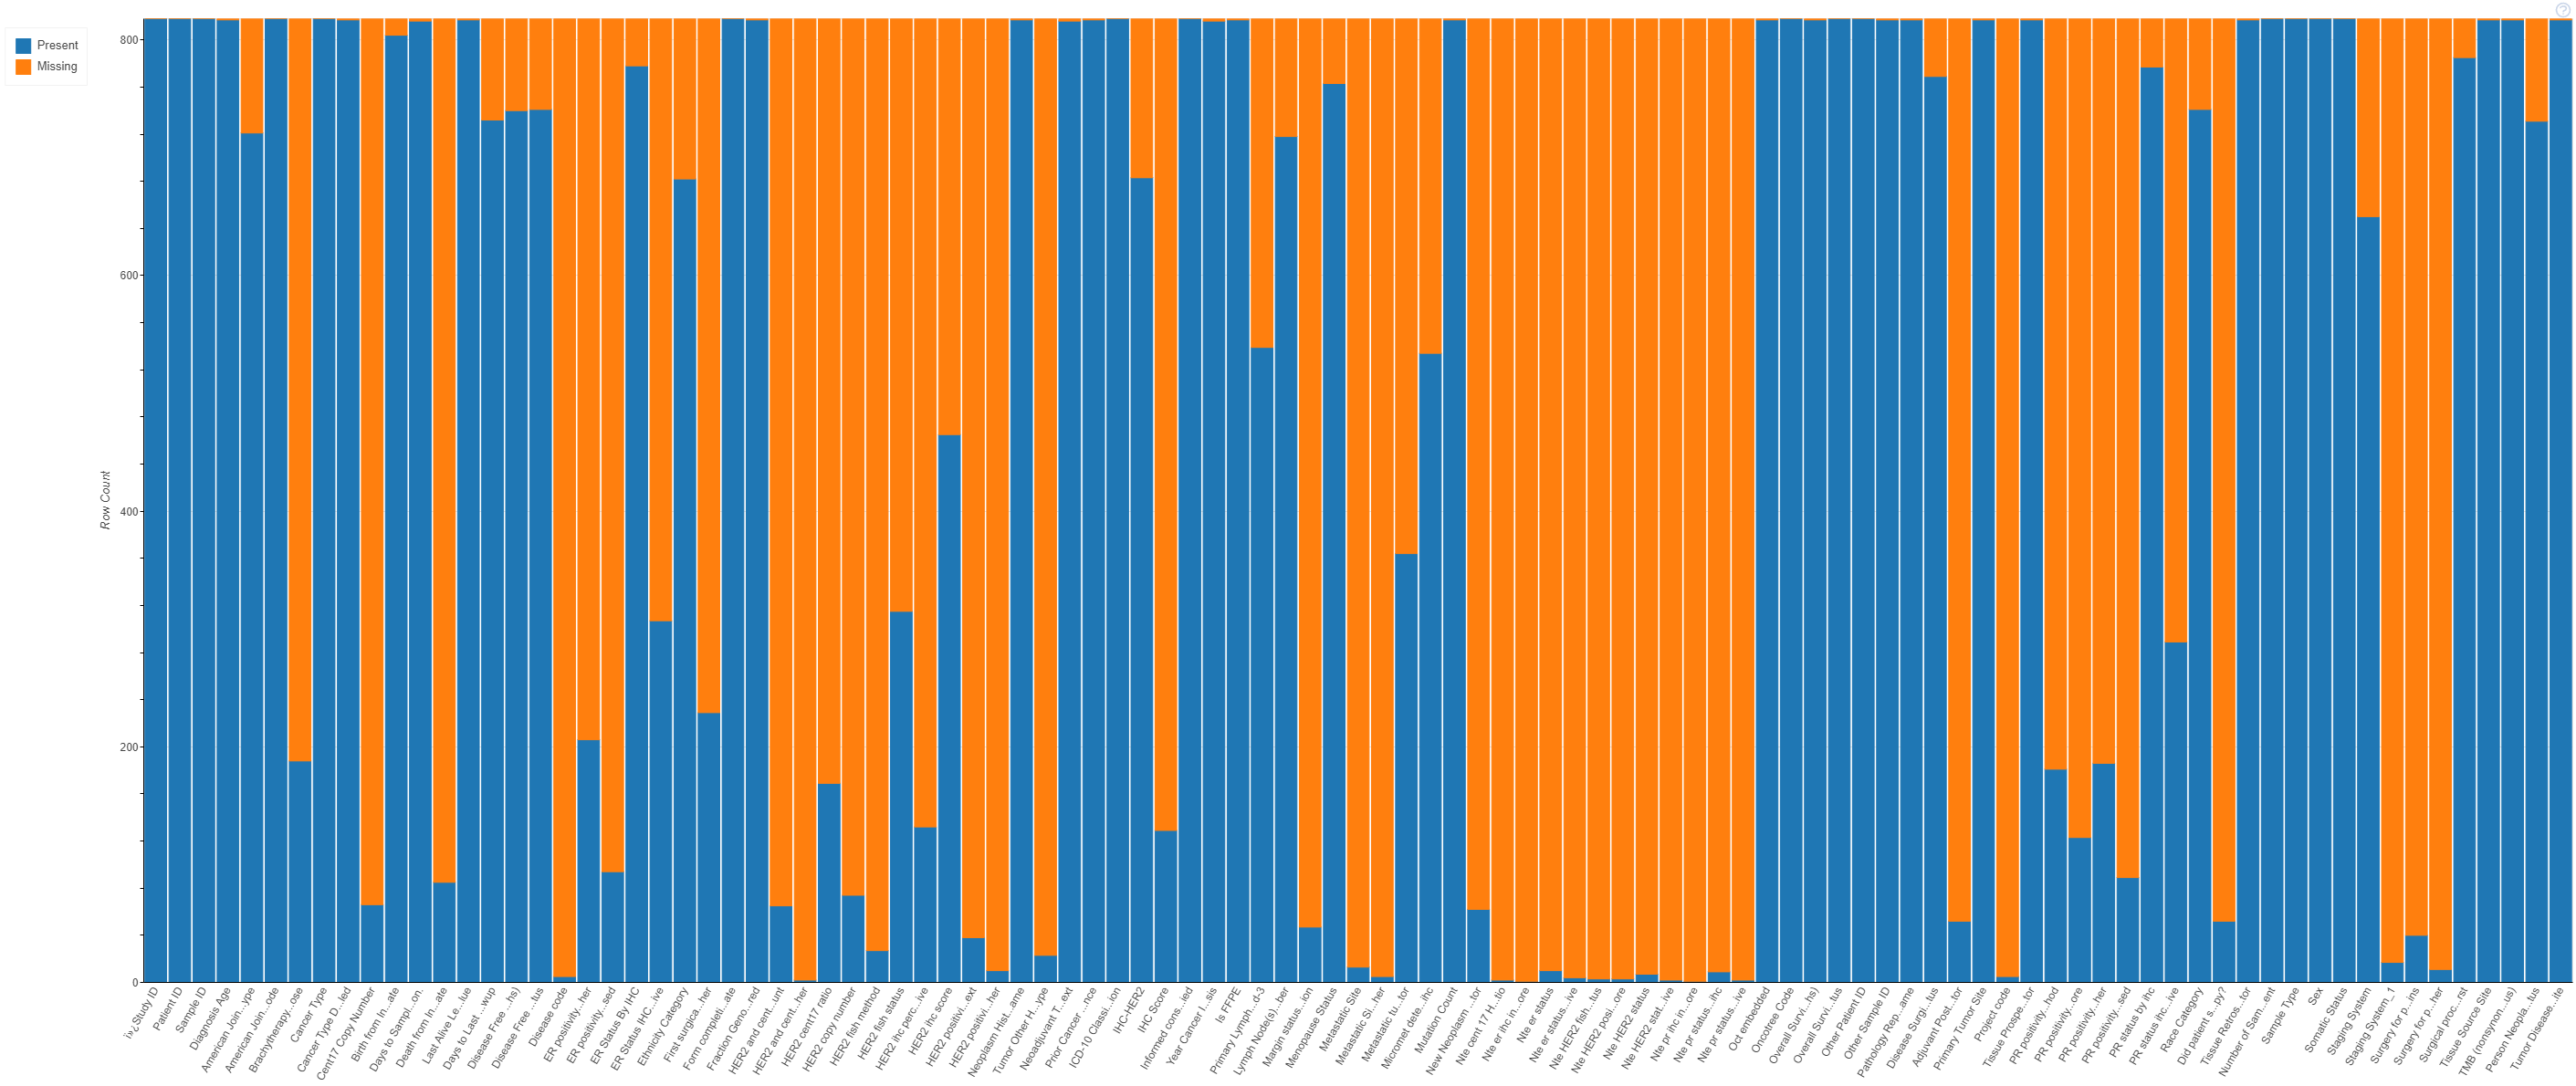
\includegraphics[width=1\linewidth]{IMAGENES/Missing_Bar_Chart}
	\caption{Datos perdidos expresados en una gráfica de barras.}
	\label{Missing_Bar_Chart}
\end{figure}

\begin{figure}[!htb]
	\centering
	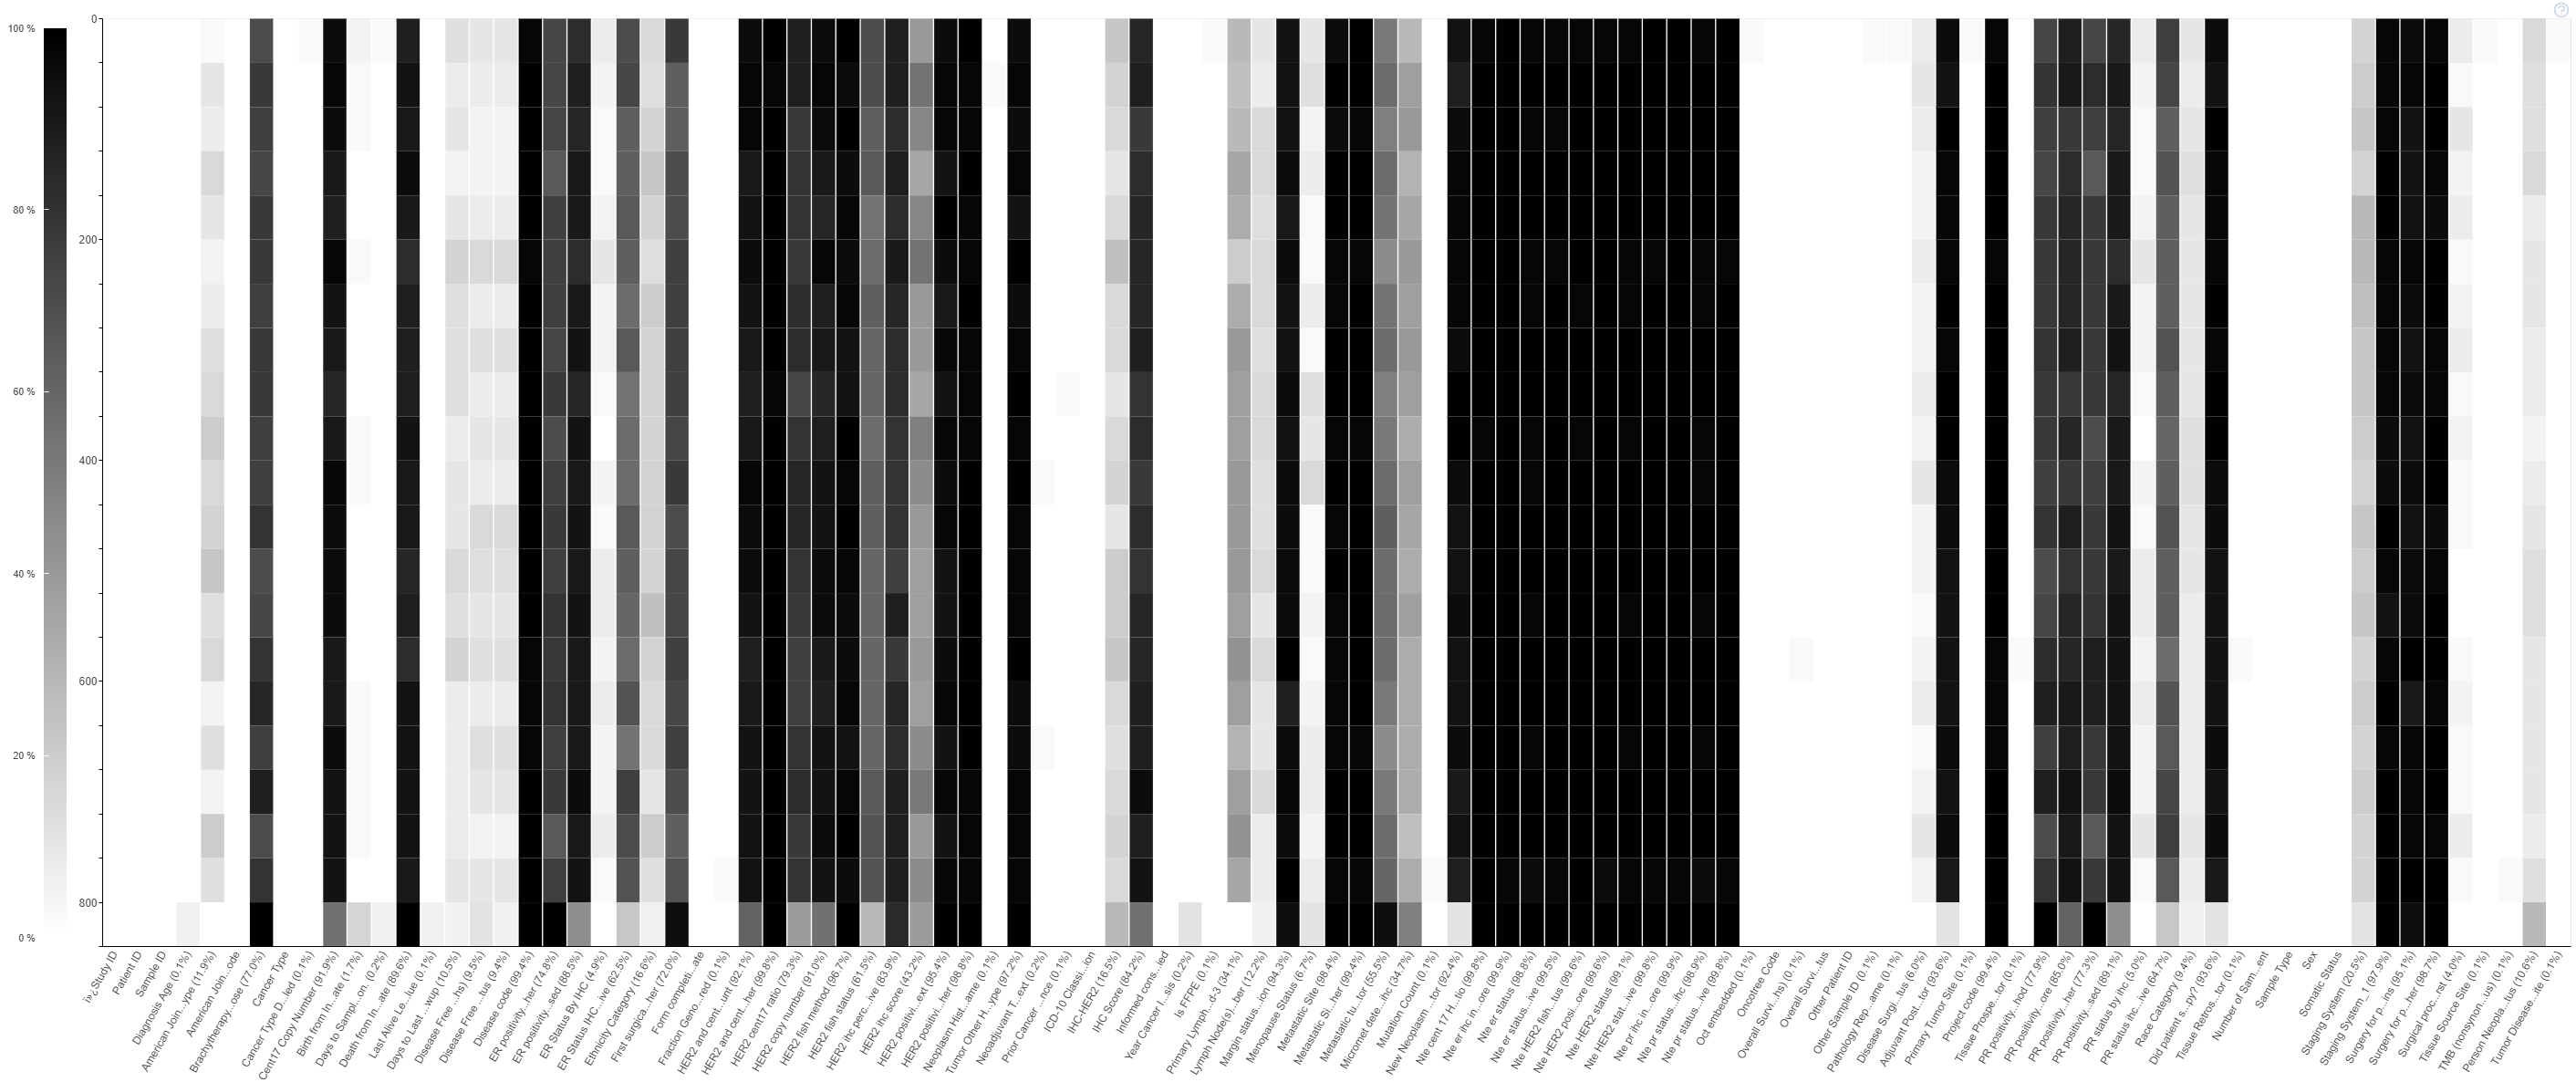
\includegraphics[width=1
	\linewidth]{IMAGENES/Missing_Spectrum}
	\caption{Datos perdidos expresados en un diagrama espectral.}
	\label{Missing_Spectrum}
\end{figure}


\subsection{Análisis Descriptivo }
En primer lugar, se realizo el respectivo análisis descriptivo para detectar cual es comportamiento de los atributos del conjunto de datos \textit{“Breast Invasive Carcinoma (TCGA, Cell 2015)”}. En la gráfica \ref{EDA} se puede observar las gráficas estadísticas unidimensionales de la 110 variables, las cuales permitieron extraer  las características mas representativas y permitieron identificar el comportamiento de los datos.

\begin{table*}[!htb]
	\footnotesize
	\begin{threeparttable}
		\caption{Conjunto de datos del Carcinoma invasivo de mama (TCGA, Cell 2015).}
		\label{Analisis_Descriptivo}
		\begin{tabular}{p{8cm} p{7cm}} \toprule	 
			\begin{center}Análisis descriptivo\end{center}             
			&\begin{center}Variable\end{center}\\ \hline
			%------------------------------------------------------	
			En segundo lugar, basados en la obtención de los atributos del conjunto de datos \textit{“Breast Invasive Carcinoma (TCGA, Cell 2015)”}, se realizo un análisis de la cantidad de datos perdidos para identificar las variables y en la etapa posterior realizar la limpieza y el pre-procesamiento de los datos de destino hacerlos consistentes y sin ningún tipo de ru	
			
			& \begin{center}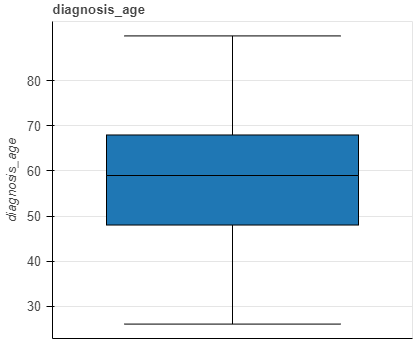
\includegraphics[width=1\linewidth]{NOTEBOOK/IMAGENES_DESCRIPTIVAS/1_diagnosis_age}\end{center}
			\\ \hline
			%------------------------------------------------------	
			En segundo lugar, basados en la obtención de los atributos del conjunto de datos \textit{“Breast Invasive Carcinoma (TCGA, Cell 2015)”}, se realizo un análisis de la cantidad de datos perdidos para identificar las variables y en la etapa posterior realizar la limpieza y el pre-procesamiento de los datos de destino hacerlos consistentes y sin ningún tipo de ru	
			
			& \begin{center}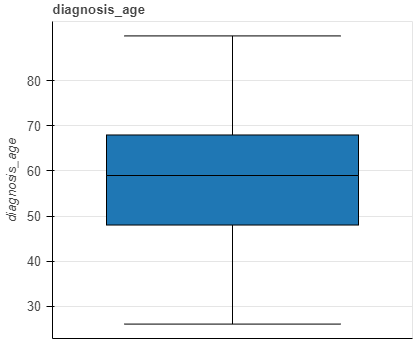
\includegraphics[width=1\linewidth]{NOTEBOOK/IMAGENES_DESCRIPTIVAS/1_diagnosis_age}\end{center}
			\\ \hline
			%------------------------------------------------------	
			En segundo lugar, basados en la obtención de los atributos del conjunto de datos \textit{“Breast Invasive Carcinoma (TCGA, Cell 2015)”}, se realizo un análisis de la cantidad de datos perdidos para identificar las variables y en la etapa posterior realizar la limpieza y el pre-procesamiento de los datos de destino hacerlos consistentes y sin ningún tipo de ru	
			
			& \begin{center}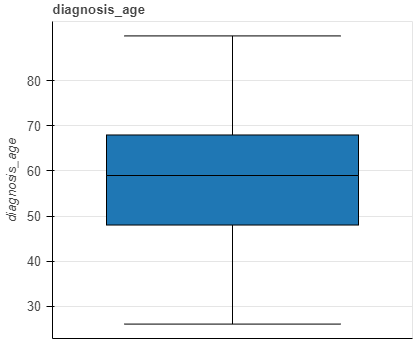
\includegraphics[width=1\linewidth]{NOTEBOOK/IMAGENES_DESCRIPTIVAS/1_diagnosis_age}\end{center}
			\\ \hline
			%------------------------------------------------------	
		\end{tabular}
	\end{threeparttable}
\end{table*}







